\section{Multitasking scheduling patterns}
\label{qnodeos:sec:multitasking_patterns}

\begin{figure*}[!htb]
\centering
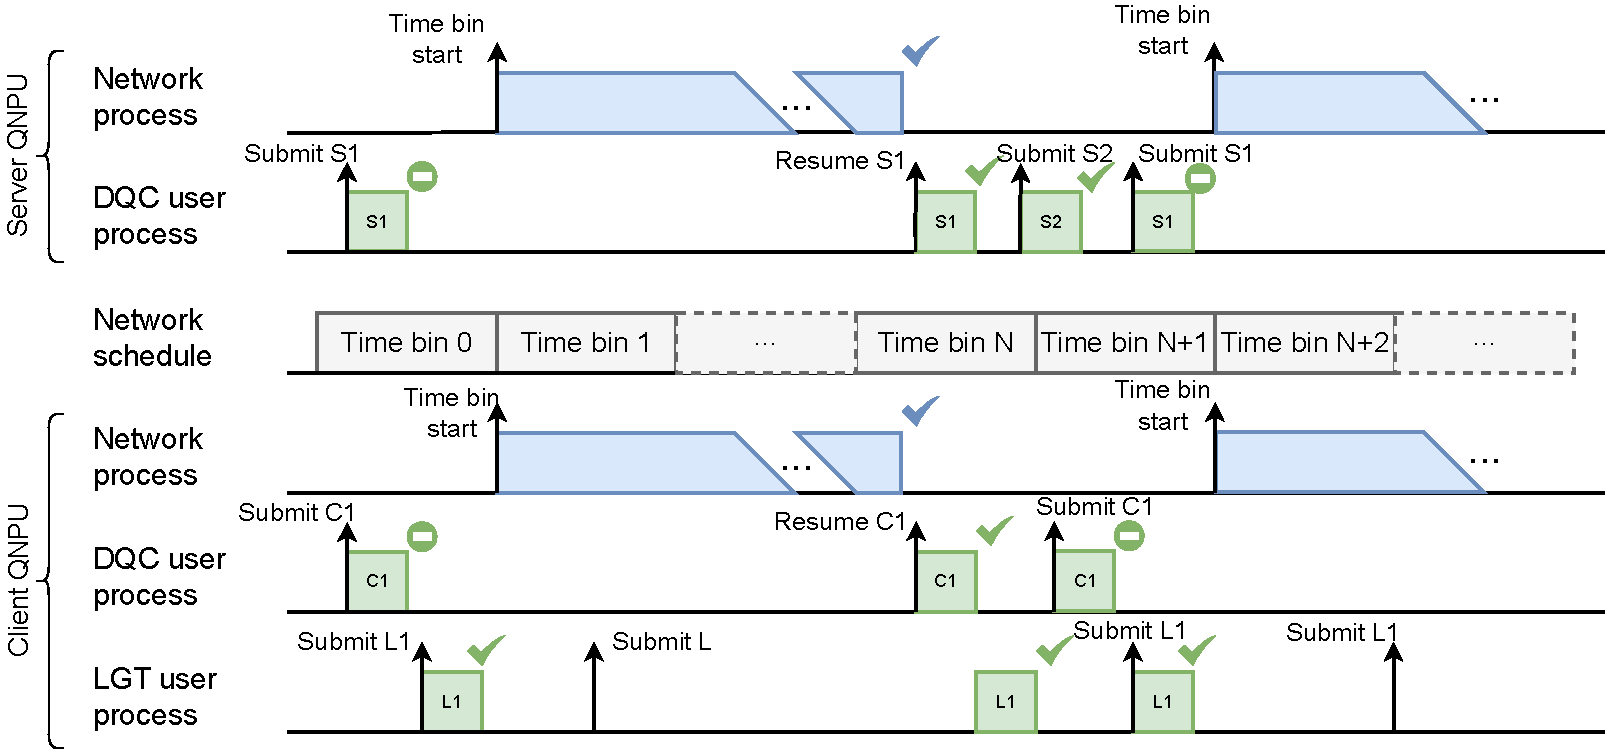
\includegraphics[width=1.0\textwidth]{figures/qnodeos/supplementary/scheduling/MT_default.pdf}
\caption{Nominal scheduling pattern on the client and server \acp{QNPU} when multitasking 1 \ac{DQC} application (on client and server) and 1 \ac{LGT} application (on client only). Pictured is a slice of time (moving to the right) in which a whole \ac{DQC} circuit execution is realized, and 3 \ac{LGT} circuit executions. Up-arrows indicate that the process becomes \textit{ready} (either since a subroutine was submitted from the \ac{CNPU}, or because a requested entangled qubit becomes available). Green blocks are \ac{NetQASM} subroutines. Blue blocks are entanglement generation. Ticks indicate completion of a subroutine (user process) or entanglement request (network process). Stop sign means the user process goes into the \textit{waiting} state. Time not to scale. Time bin length is 10\,ms. Duration of L1 is $\approx$2.4\,ms. Duration of entanglement generation is non-deterministic. On the server \ac{QNPU} the following happens. S1 arrives from \ac{CNPU}; \ac{DQC} user process becomes \textit{ready}. \ac{DQC} user process is activated and executes S1. The entanglement instruction inside S1 is reached; entanglement request is sent to network stack; \ac{DQC} user process becomes \textit{waiting}. When time bin 1 starts, network process becomes \textit{ready}. There is a pending entanglement request, so network process is activated; \ac{QDevice} attempts entanglement until success (after non-deterministic number of time bins, blue tick). Requested entangled qubit is available: \ac{DQC} user process becomes \textit{ready} again; is activated; executes S1 until completion; becomes \textit{idle}. \ac{QNPU} receives subroutine S2 from \ac{CNPU}; activates \ac{DQC} user process; executes S2 until completion. At this point, the \ac{QNPU} completed execution of the current repetition of the \ac{DQC} circuit. \ac{QNPU} then receives again a subroutine S1 (for the next \ac{DQC} circuit iteration), and the same pattern repeats. On the client \ac{QNPU} the following happens. C1 arrives from \ac{CNPU}; \ac{DQC} user process becomes \textit{ready}. \ac{DQC} user process is activated and executes C1. The entanglement instruction inside C1 is reached; entanglement request is sent to network stack; \ac{DQC} user process becomes \textit{waiting}. L1 arrives from \ac{CNPU}; \ac{LGT} user process becomes \textit{ready}. \ac{LGT} user process is activated; fully executes L1. When time bin 1 starts, network process becomes \textit{ready}. There is a pending entanglement request, so network process is activated; \ac{QDevice} attempts entanglement until success (blue tick). While network process is active, another L1 block arrives from \ac{CNPU} (for next \ac{LGT} circuit iteration) so \ac{LGT} user process becomes \textit{ready}. \ac{LGT} user process is not activated since network process is still running. Upon entanglement success, requested qubit is available; \ac{DQC} user process is activated to complete C1. \ac{QNPU} has now completed execution of the current repetition of the \ac{DQC} circuit. \ac{LGT} user process is activated to execute L1 which was still pending. The same pattern repeats.
}
\label{qnodeos:fig:multitasking-default}
\end{figure*}

\clearpage

\begin{figure*}
\centering
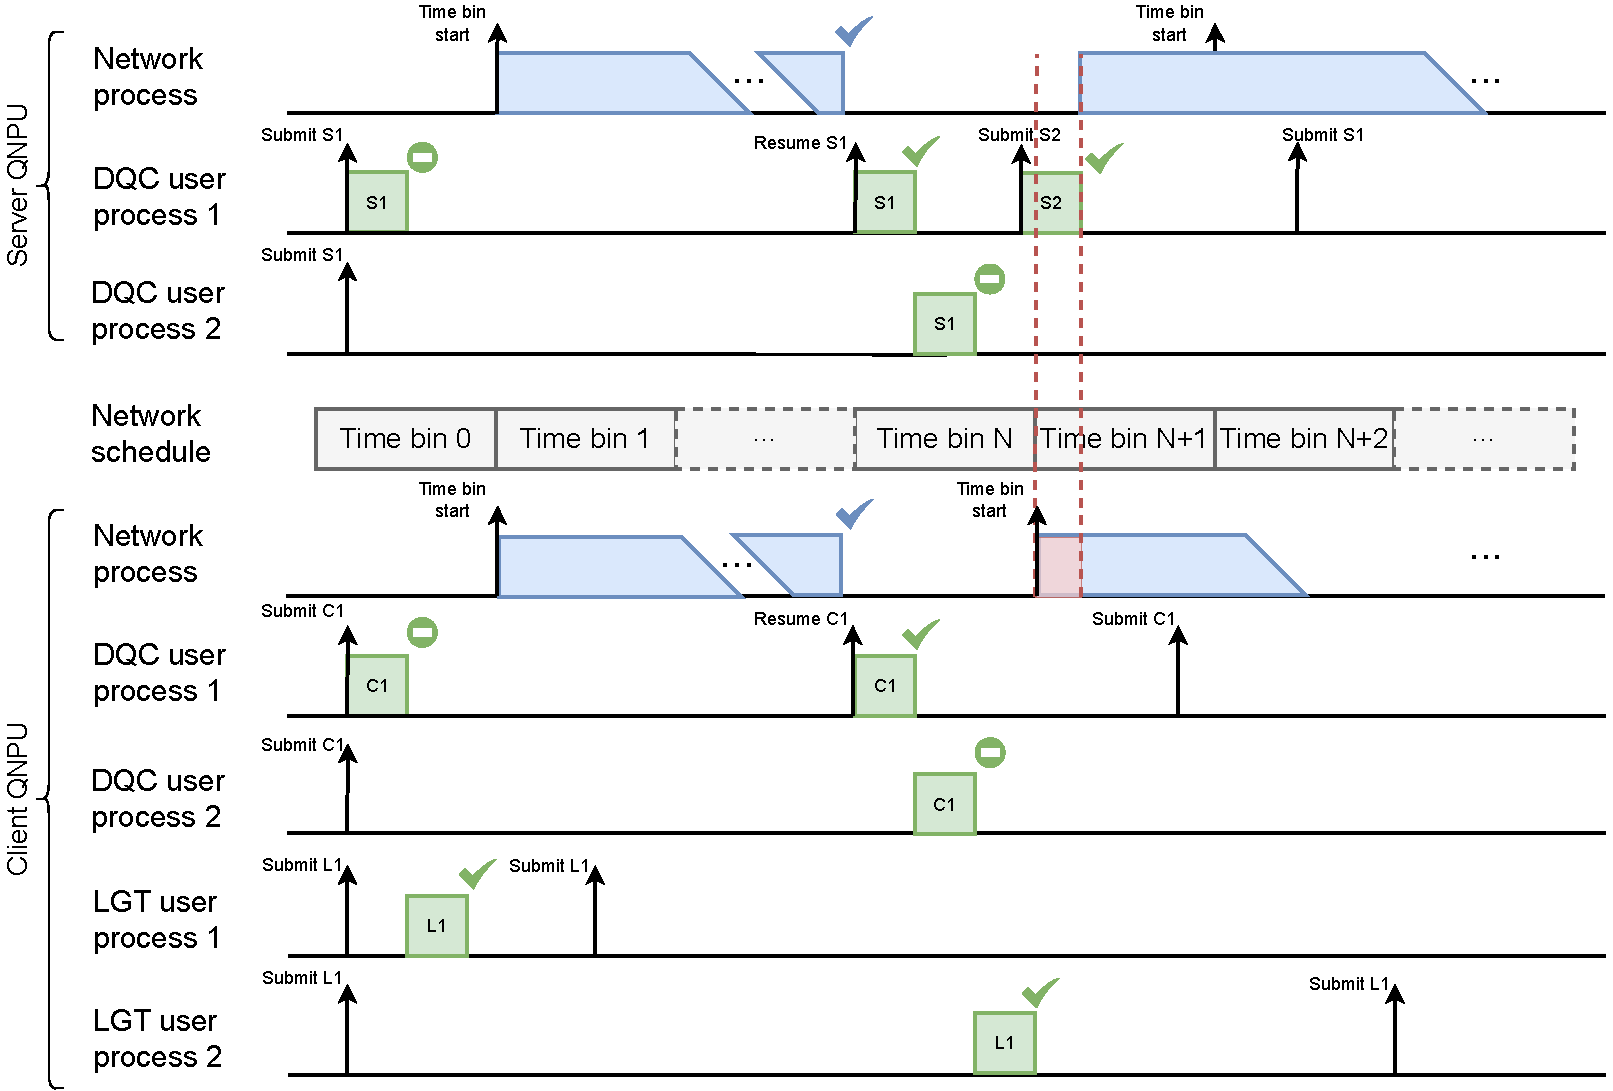
\includegraphics[width=1.0\textwidth]{figures/qnodeos/supplementary/scheduling/MT_2_apps.pdf}
\caption{Example scheduling pattern of scenario with 2 \ac{DQC} applications and 2 \ac{LGT} applications (the symbol and color coding is the same as in~\cref{qnodeos:fig:multitasking-default}). In this case, the client needs to wait (red shared area) for the server to finish S2 of \ac{DQC} user process 1, before they can do entanglement generation for \ac{DQC} user process 2. Scenario: 2 \ac{DQC} applications (A1 and A2) are concurrently executed (A1: \ac{DQC}-server program executed by server \ac{DQC} user process 1 and \ac{DQC}-client program executed by client \ac{DQC} user process 1; A2: \ac{DQC}-server program executed by server \ac{DQC} user process 2 and \ac{DQC}-client program executed by client \ac{DQC} user process 2). Client and server successfully create entanglement for some \ac{DQC} circuit execution $i$ for A1 (just after time bin $N$ starts). Client finishes C1 for user process 1, and meanwhile the server finishes S1 for user process 1. The client has completed its part of \ac{DQC} circuit execution $i+1$ for A1, but the server still needs to wait for S2 from the \ac{CNPU}. Then, the client executes C1 for user process 2, which is the start of circuit execute $j$ for A2; user process 2 becomes waiting. Meanwhile the server executes S1 for user process 2 which becomes waiting. The client needs to wait until the start of the next time bin ($N+1$) until it can activate the network process to handle the request. In the meantime, it can execute an L1 block. Time bin $N+1$ starts and the client handles the request. However, the server has received S2 for execution $i$ of A1, and starts executing it just before the time bin starts. Only after finishing it, the server can start the network process, which picks up the request for A2. While S2 is executing, the client \ac{QDevice} tries to do entanglement attempts, but gets entanglement sync failures~\cref{qnodeos:sec:qdevice-sync} since the server \ac{QDevice} is busy with S2.}
\label{qnodeos:fig:multitasking-2-apps}
\end{figure*}

\clearpage

\begin{figure*}
\centering
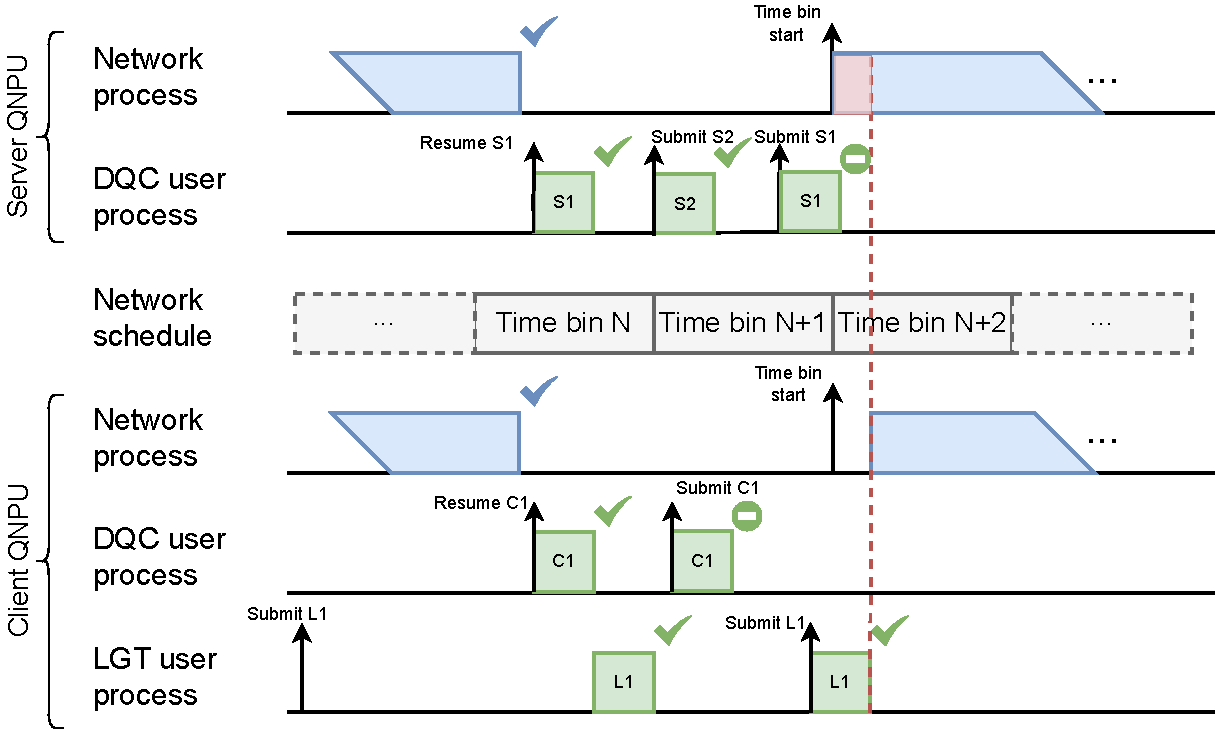
\includegraphics[width=1.0\textwidth]{figures/qnodeos/supplementary/scheduling/MT_wait_on_client.pdf}
\caption{Example scheduling pattern of multitasking one \ac{DQC} application (on client and server) and one \ac{LGT} application (on client only), where the server must wait for client to finish its \ac{LGT} user process (red area); the symbol and color coding is the same as in~\cref{qnodeos:fig:multitasking-default}. At the start of time bin $N+1$, the server activates the network process to handle the request that was put by the previous S1 execution. However the client only starts some time later during the time bin, since it first needs to finish executing L1 for the \ac{LGT} user process.}
\label{qnodeos:fig:multitasking-wait-on-client}
\end{figure*}